\begin{columns}
    \column{0.5}
    \block{Molecular dynamic (MD) simulation} {
        
        \vspace{0.5cm}

        \begin{itemize}
            \item \textbf{Number of atoms:} between 10 and 5000 atoms ;
    
            \vspace{0.5cm}
    
            \item \textbf{Simulation time:} between 0.5 ns and 5 ns ;
            
            \vspace{0.5cm}
    
            \item \textbf{Composition:} between 0\% and 100\% of \textcolor{colorAg}{\textbf{Ag}} atoms (the rest being \textcolor{colorCo}{\textbf{Co}} atoms) ;

            \vspace{0.5cm}

            \item \textbf{Initial temperature:} between 1500 K and 2500 K ;

            \vspace{0.5cm}

            \item \textbf{Final temperature:} 300 K ;

            \vspace{0.5cm}

            \item \textbf{Canonical ensemble:} Nosé-Hoover thermostat + linear decrease of the temperature            
                
                \vspace{1cm}
            
                \begin{equation}
                    T(t) = \frac{T_{\text{final} - T_\text{initial}}}{t_{\text{final}}}t + T_\text{initial}
                \end{equation}            

            \vspace{1.5cm}

            \item \textbf{Interatomic potential:} TBSMA (Tight-Binding Second Moment Approximation) 
                
                \vspace{1cm}
            
                \begin{equation}
                    \mathcal{U} = \sum^N_{i=1} \left[\sum_{j\ne i}^NAe^{-p(r_{ij}/r_0 - 1)} -\sqrt{\sum_{j\ne i}^N\xi^2e^{-2q(r_{ij}/r_0 - 1)}}~\right]
                \end{equation}
        \end{itemize}
        
        \vspace{2.5cm}
        
        \begin{center}
            \begin{tikzpicture}
                % Image 1 (nœud "image1")
                \node[anchor=west, inner sep=0] (image1) at (0,0) {
                    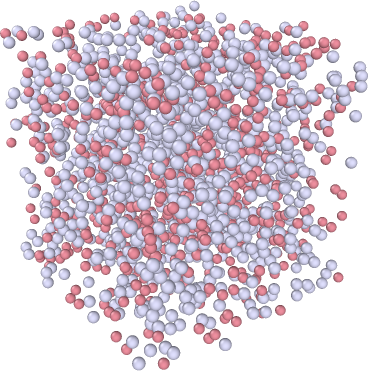
\includegraphics[width=0.25\linewidth]{Figure/MD/md_init.png}
                };

                % Image 2 (nœud "image2") à droite de l'image 1
                \node[anchor=west, inner sep=0, xshift=0.5\linewidth] (image2) at (0,0) {
                    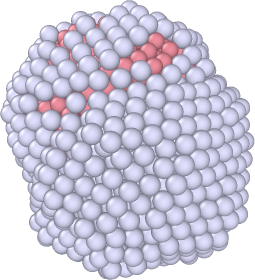
\includegraphics[width=0.15\linewidth]{Figure/MD/md_final.png}
                };

                % Légendes sous les images (optionnel)
                \node[anchor=north, align=center] at (image1.south) {Initial configuration};
                \node[anchor=north, align=center] at (image2.south) {Final configuration};

                % Flèche entre les deux images
                \draw[->, thick] (image1.east) -- (image2.west);
            \end{tikzpicture}
        \end{center}
    }
    \column{0.5}
    \block{Creation of the dataset} {
        
        \vspace{0.5cm}

        \textbf{Nanoalloys dataset}

        \vspace{1cm}

        The \textbf{dataset of nanoalloys} is generated by using \textbf{MD simulations with random parameters}, as described in the "Molecular dynamic (MD) simulation" block.
        
        \vspace{0.5cm}

        \begin{itemize}
            \item \textbf{Number of data:} 48000 data points ;
            
            \vspace{0.5cm}
            
            \item \textbf{Large diversity of data} thanks to the random parameters of the MD simulations.
        \end{itemize}

        \vspace{1.5cm}

        \begin{center}
            \begin{tikzpicture}
                % Image 1 (nœud "image1")
                \node[anchor=west, inner sep=0] (image1) at (0,0) {
                    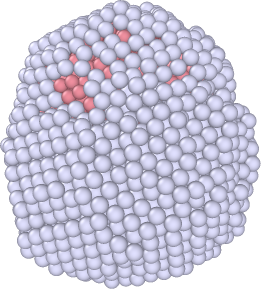
\includegraphics[width=0.15\linewidth]{Figure/particle_exemple.png}
                };

                % Image 2 (nœud "image2")
                \node[anchor=west, inner sep=0, xshift=0.2\linewidth] (image2) at (0,0) {
                    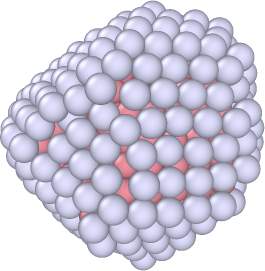
\includegraphics[width=0.15\linewidth]{Figure/particle_exemple2.png}
                };

                % Image 3 (nœud "image3")
                \node[anchor=west, inner sep=0, xshift=0.4\linewidth] (image3) at (0,0) {
                    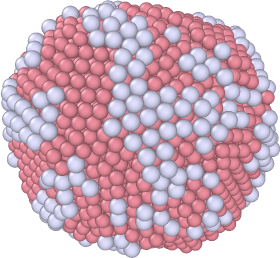
\includegraphics[width=0.15\linewidth]{Figure/particle_exemple3.png}
                };

                % Image 4 (nœud "image4")
                \node[anchor=west, inner sep=0, xshift=0.6\linewidth] (image4) at (0,0) {
                    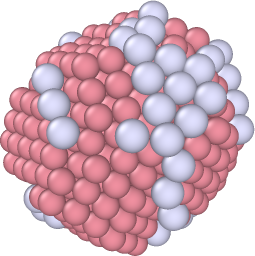
\includegraphics[width=0.15\linewidth]{Figure/particle_exemple4.png}
                };
            
                \node[anchor=north, align=center, yshift=-0.025\linewidth] at (current bounding box.south) {Examples of the dataset};
            \end{tikzpicture}
            
        \end{center}

        \vspace{2cm}

        \textbf{HRTEM images dataset}

        \vspace{1cm}

        The \textbf{dataset of HRTEM images} is generated by using the \textbf{DrProbe} software to simulate the HRTEM images of nanoalloys in the nanoalloysdataset.
        
        \vspace{1.5cm}

        \begin{center}
            \begin{tikzpicture}
                % Image 1 (nœud "image1")
                \node[anchor=west, inner sep=0] (image1) at (0,0) {
                    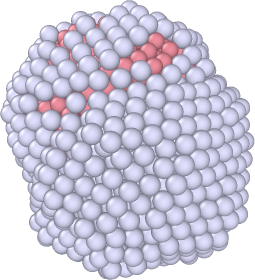
\includegraphics[width=0.15\linewidth]{Figure/MD/md_final.png}
                };

                % Image 2 (nœud "image2") à droite de l'image 1
                \node[anchor=west, inner sep=0, xshift=0.4\linewidth] (image2) at (0,0) {
                    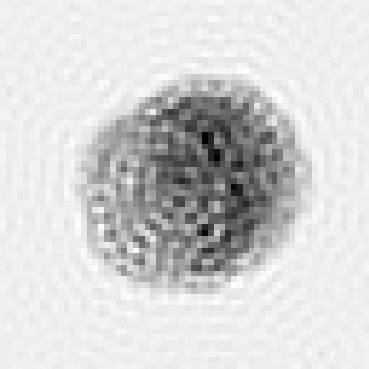
\includegraphics[width=0.25\linewidth]{Figure/1_1.png}
                };

                % Légendes sous les images (optionnel)
                \node[anchor=north, align=center] at (image1.south) {Sample};
                \node[anchor=north, align=center] at (image2.south) {HRTEM image};

                % Flèche entre les deux images
                \draw[->, thick] (image1.east) -- (image2.west);
                \node[anchor=south, align=center, font=\small] at ([yshift=0.1cm]$(image1.east)!0.5!(image2.west)$) {\textbf{DrProbe}};
            \end{tikzpicture}
        \end{center}    
    }
\end{columns}